\section{Study 3: Password Selection}
% ALINE
% GOALS
As a final step in our ``password personality'' exploration, we ran an online survey. Having investigated preferences for policies and the perception of passwords, the main goal of the third study was to evaluate potential associations between personality and password \textit{selection}. To overcome some of the limitations of the previous study, we hoped to increase the sample size and reduce the number of items during the study. Moreover, further answers about the participants' explanations and motivations were considered to better understand the weight of personality factors. We determined the following research questions: 1) Are there correlations between password features (topology) and personality traits? 2) Do certain facets of personality shine through in password management behavior, e.g. the tendency to write down passwords?

\subsection{Procedure and Tools}
The study was designed to take no more than ten minutes. The briefing page informed participants about the purpose of the study and data disclosure policies. After acknowledging the conditions of participation, respondents were asked to create a password. To boost ecological validity, we provided a fictitious but realistic scenario \cite{Komanduri2011OfPasswordsAndPeople}. The task was to come up with a new password for a new email account that they were going to use as their main address. Further, the instruction pointed out that the incentive would only be paid of if the participants chose a password they could recall later on. A \textit{basic8} policy was enforced, as it is one of the most representative policies in the wild (see chapter \ref{chap:policies_reuse}). This loose policy would also allow for both very complex and rather simple passwords, which could be associated with personality traits. Having successfully confirmed the password, respondents were taken to a questionnaire about demographics, just like in the first two studies. 

Next, participants completed the BFI-K questionnaire consisting of 21 items that have to be rated on a 5-point scale. We opted not to use the 50-item inventory for the sake of saving time. We added an item that served as an attention check. It asked to respond to this item with ``disagree''. Failure to follow this instruction allowed us to drop the response from the dataset. The resulting 22 items were shuffled to avoid sequence effects. 

Afterwards, we surveyed respondents about their password management behaviors and preferences. We used multiple-choice and open responses to collect qualitative, self-reported data. For instance, we wanted to know how they cope with multiple accounts or how they reuse passwords. The survey concluded with a recall task, where participants provided their initially chosen password. They could try as often as they liked, and the number of attempts were recorded. In case they were unable to recall their password, they could proceed anyhow and take part in the lottery. If they chose to provide an email address in the final step, this data was stored separately from the questionnaire data to avoid privacy issues. 

\subsection{Recruitment and Sample}
Participants were invited via a university newsletter, and snowballing the link via personal connections and posts on social networks. The questionnaire was in German and participants were screened about their command of the German language. We instructed participants to take the survey on a desktop. 
%TODO aline says 184 but the data set is smaller :-/ ?
%all the following numbers are from the smaller data set.
184 people completed the survey, but we had to drop the responses of 8 participants because their reponse timings were too unrealistic. From the 176 remaining respondents, 89 were male, 86 female and 1 preferred not to answer. 116 were students, i.e. a rather high proportion (66\%). Consequently, the average age was 25 years (range [16;55], $SD$=6, $Md$= 24). 67 (38\%) reportedly had an IT-background. 129 respondents chose to participate in the raffle for shopping vouchers. 

\subsection{Limitations}
\todo{Password selection not realistic / attention check item was badly placed and not well explained. 30 feedback emails.}

\subsection{Results}
% descriptives
The resulting passwords had a median-length of 10 characters ([8;22]), i.e. many participants went beyond the minimum requirement. Figure \ref{fig:personality:study3:metrics-overview} visualizes additional metrics that show that passwords were stronger than expected. Moreover, overall internal consistency was at $\alpha=0.65$, thus slightly below the bar. Subscales for each trait were fairly consistent. In the following, we try to fit generalized additive models to the data using big-five trait scores as covariates. 

\begin{figure}[tbph]
	\centering
	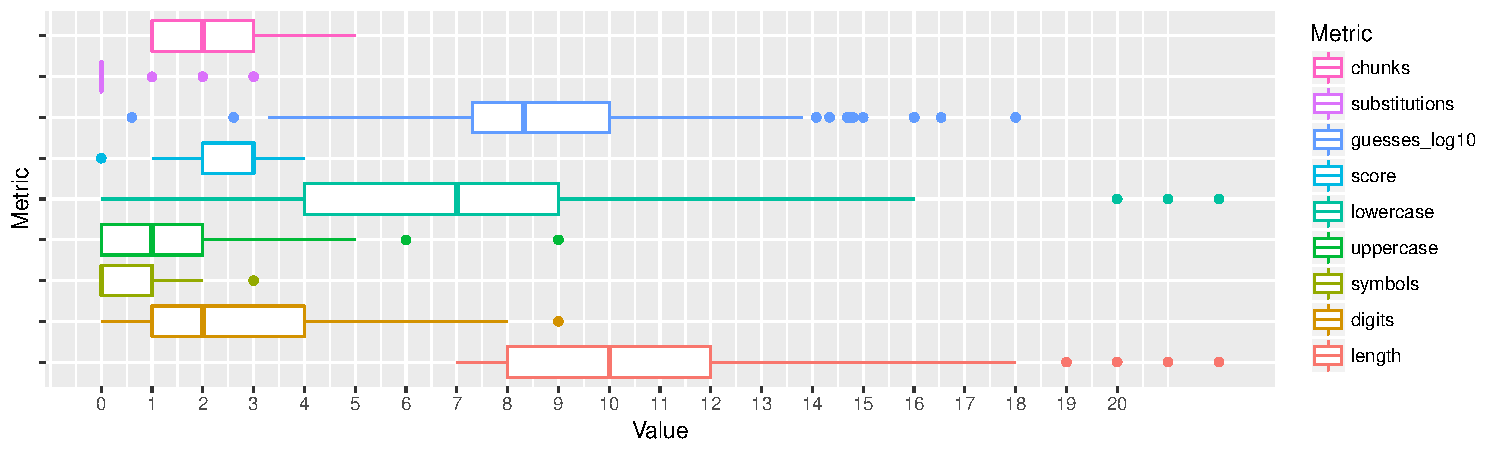
\includegraphics[width=1\linewidth]{figures/personality/study3-metrics-overview}
	\caption{\label{fig:personality:study3:metrics-overview} Zxcvbn metrics for user selected passwords.}
\end{figure}

% maximum R-sq 
\subsubsection{Password Composition}
%TODO aline's data suggests that all this was associated with agreeableness, instead of neuroticism, but I found a labelling error. discuss!
First, we use zxcvbn metrics as response variables, and explore marginal associations with big five traits. As before, we include age, gender and IT-background as control covariates. We found that only password length was (significantly) associated with B5-traits: Participants with higher \textit{neuroticism} scores tended to create shorter passwords ($\beta = -0.21$), using fewer lower-case letters as a side effect ($\beta = -0.19$). A second corollary was that passwords from participants scoring high on neuroticism were divided into fewer chunks ($\beta=-0.26$). However, it is hard to read this result, because even very long random passwords consist of only one matching sequence (``bruteforce''). 
%control variables and model fit. 
Having an IT background, on the contrary, was positively associated with password length ($\beta = 0.21$). A one-tailed Mann-Whitney test confirms this ($W=4204$,\pvallt{0.04}). Consequently, password strength was higher if participants had an IT background ($\beta=0.19$). None of the models however, achieved considerable fit: the maximum R-squared (adjusted) value was \Rsqadj{0.13} (for the number of symbols as target variable). We tried to achieve a better fit by performing a principal component analysis. This was not effective, either. We conclude that password selection analyzed with standard quantitative metrics is only very slightly predictable by personality profiles. 
%OPTIONAL point much smaller R-sq than in second study. 

%\subsection{Selection Strategies} -- no noteworthy association so we leave this out. and also I don't understand how Aline approached this. the categories seem too arbitrary. 

\subsubsection{Password Management Strategies}
Respondents freely reported reusing passwords (88.4\%), and 65.34\% said to categorize their passwords. Memorizing passwords was the preferred strategy for 109 participants, followed by notes on paper or a file ($n$=43). Using a password manager was the least favored option ($n=24$).

% binary -- logit model ``write down'': yes no
We created generalized additive logit models for every management strategy, i.e. binary outcomes like ``Using a password manager'': 1 (true) or 0 (false). 

Since the percentage of participants reusing passwords is so high, influence by personality traits was unlikely to be detected. Consequently, none of the associations was flagged as significant for ``reuse''. However, older participants were more likely to reuse passwords as shown in Figure \ref{fig:personality:study3:age-openness-coping-all}. Participants with an IT background reported less password reuse ($\beta=-1.97$). We can observe another interesting aspect in Figure \ref{fig:personality:study3:age-openness-coping-all} which depicts associations between coping strategies and age, respectively Openness scores. Although not flagged as significant, age and openness show a positive tendency towards using a password manager. Similarly, memorizing passwords is less likely to be found with older and more open participants. Generally, memorizing passwords seems to be the only unfavorable coping strategy for older participants. 
\begin{figure}[tbph]
	\centering
	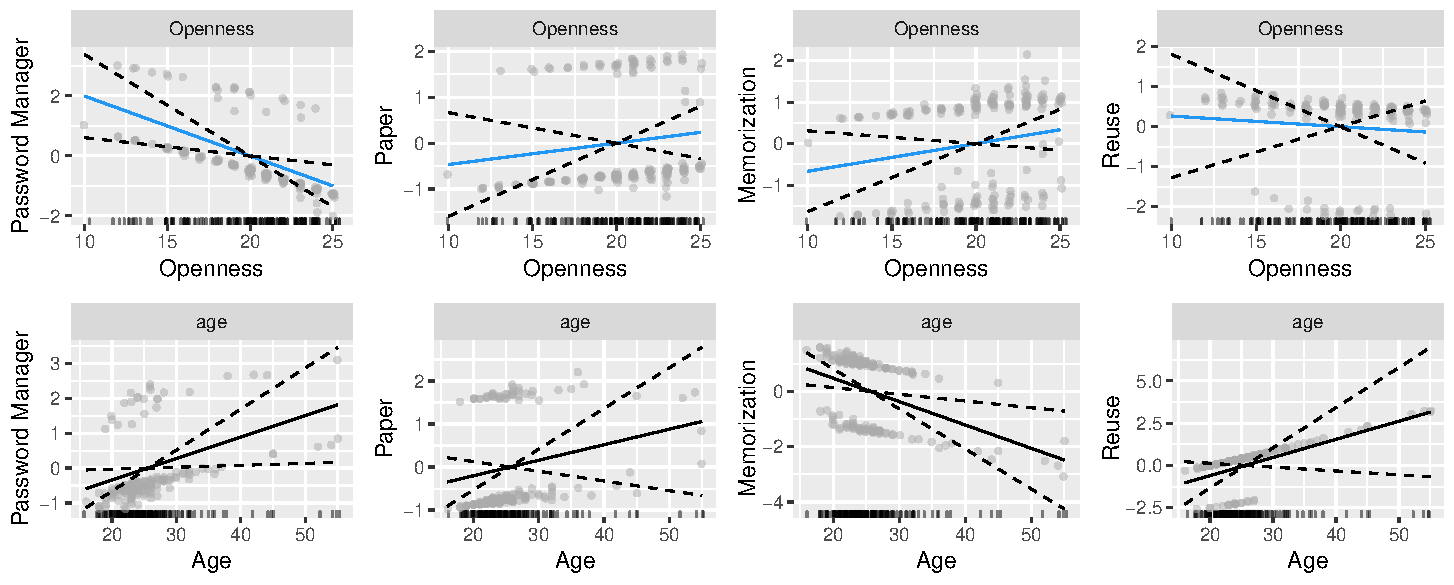
\includegraphics[width=1\linewidth]{figures/personality/age-openness-coping-all}
	\caption{\label{fig:personality:study3:age-openness-coping-all}Age and Oppenness model plots for the three coping strategies password manager, paper-notes and memorization.}
\end{figure}

\subsubsection{Memorability}
Only 18 out of 176 participants (10\%) failed to recall the newly created password at the end of the survey. Thus, associations with personality traits were unlikely.

\subsubsection{Other findings}
One participant P48claimed that their password (\texttt{!Q\"W3e4}) was not based on keyboard patterns. Zxcvbn also failed to recognize the pattern, because it only is obvious on a keyboard with a German layout where the quotation marks are entered with Shift+2. 

Internal consistency analysis with the alpha function suggested to reverse neuroticism items to increase reliability. This is an odd finding, but could be due to chance. 


\subsection{Learnings}
Password length/strength marginally associated with Neuroticism

binary outcome (memorability) needs a larger sample 
